\chapter{Le cycle cellulaire et la mitose}\label{ch:g11:cell-cycle-mitosis}

Écrasez sous une lamelle l'extrémité d'une racine d'oignon, colorez-la
et regardez~: parmi des centaines de \omterm{def:g10:cells-common-unit:cell}{cellules} tranquilles à \omterm{def:g10:cells-common-unit:organelle}{noyau} rond,
quelques-unes montrent autre chose --- des bâtonnets sombres en forme
de X rassemblés au milieu de la \omterm{def:g10:cells-common-unit:cell}{cellule}, ou deux lots de bâtonnets
écartés vers les extrémités, ou deux petits \omterm{def:g10:cells-common-unit:organelle}{noyaux} avec une paroi qui
se forme entre eux. Vous observez des divisions cellulaires saisies à
des moments différents, dans un tissu qui croît d'un millimètre par
jour. Chacune de ces divisions remet deux lots complets et identiques
de \omterm{def:g10:universal-dna:information}{chromosomes} à deux \omterm{def:g10:cells-common-unit:cell}{cellules} filles. Ce chapitre suit une \omterm{def:g10:cells-common-unit:cell}{cellule} sur
un cycle entier, et examine de près l'heure pendant laquelle les
\omterm{def:g10:universal-dna:information}{chromosomes} sont répartis.

\section{Le cycle cellulaire}

\begin{definition}[Cycle cellulaire]\label{def:g11:cell-cycle-mitosis:cycle}
Le \emph{cycle cellulaire}\index{cycle cellulaire} est la suite des
événements qui vont de la naissance d'une \omterm{def:g10:cells-common-unit:cell}{cellule}, par division, à sa
propre division en deux. Il comprend l'\emph{interphase}, pendant
laquelle la \omterm{def:g10:cells-common-unit:cell}{cellule} croît et copie son \omterm{def:g10:universal-dna:information}{ADN}, et la \emph{phase M},
pendant laquelle le \omterm{def:g10:cells-common-unit:organelle}{noyau} se divise (la \emph{mitose}\index{mitose})
puis le \omterm{def:g10:cells-common-unit:cell}{cytoplasme} (la \emph{cytodiérèse}). L'interphase compte trois
parties~: $\mathrm{G_1}$ (croissance), S (\omterm{def:g11:dna-replication:replication}{réplication de l'ADN},
\cref{ch:g11:dna-replication}) et $\mathrm{G_2}$ (préparation de la
division).
\end{definition}

\begin{omfigure}
\begin{tikzpicture}[font=\small]
  % pie: G1 11h, S 8h, G2 4h, M 1h  (24h) -> angles: G1 165°, S 120°, G2 60°, M 15°
  \fill[omDef!30] (0,0) -- (90:2.2) arc (90:-75:2.2) -- cycle;
  \fill[omProp!35] (0,0) -- (-75:2.2) arc (-75:-195:2.2) -- cycle;
  \fill[omMeth!35] (0,0) -- (-195:2.2) arc (-195:-255:2.2) -- cycle;
  \fill[omThm!50] (0,0) -- (-255:2.2) arc (-255:-270:2.2) -- cycle;
  \draw[thick] (0,0) circle (2.2);
  \foreach \a in {90,-75,-195,-255} \draw[thick] (0,0) -- (\a:2.2);
  \node at (10:1.3) {$\mathrm{G_1}$};
  \node at (-135:1.3) {S};
  \node at (-225:1.35) {$\mathrm{G_2}$};
  \node[anchor=south east] at (-262:2.35) {M};
  \node[anchor=west, align=left] at (2.6,1.3) {$\mathrm{G_1}$~: croissance, environ \qty{11}{h}};
  \node[anchor=west, align=left] at (2.6,0.5) {S~: réplication de l'ADN, \qty{8}{h}};
  \node[anchor=west, align=left] at (2.6,-0.3) {$\mathrm{G_2}$~: préparation, \qty{4}{h}};
  \node[anchor=west, align=left] at (2.6,-1.1) {M~: mitose et cytodiérèse, \qty{1}{h}};
  \draw[->, thick] (100:2.5) arc (100:130:2.5);
\end{tikzpicture}

{\small Le \omterm{def:g11:cell-cycle-mitosis:cycle}{cycle cellulaire} d'une \omterm{def:g10:cells-common-unit:cell}{cellule} humaine en division ordinaire,
environ 24 heures. L'interphase ($\mathrm{G_1}$, S, $\mathrm{G_2}$) en
occupe 23~; la division elle-même, une seule. Beaucoup de \omterm{def:g10:cells-common-unit:cell}{cellules}
quittent le cycle après $\mathrm{G_1}$ et ne se divisent plus jamais.}
\end{omfigure}

\begin{proposition}[L'ADN au fil du cycle]\label{prop:g11:cell-cycle-mitosis:dna}
Appelons $q$ la quantité d'\omterm{def:g10:universal-dna:information}{ADN} d'un \omterm{def:g10:cells-common-unit:organelle}{noyau} juste après la division. Elle
reste à $q$ pendant $\mathrm{G_1}$, monte régulièrement jusqu'à $2q$
pendant S à mesure que les \omterm{def:g10:universal-dna:information}{chromosomes} sont copiés, reste à $2q$
pendant $\mathrm{G_2}$ et la première partie de la \omterm{def:g11:cell-cycle-mitosis:cycle}{mitose}, et retombe à
$q$ dans chaque \omterm{def:g10:cells-common-unit:organelle}{noyau} fille à la fin de la \omterm{def:g11:cell-cycle-mitosis:cycle}{mitose}. Le nombre de
\omterm{def:g10:universal-dna:information}{chromosomes} ne change pas pendant S~: chaque \omterm{def:g11:cell-cycle-mitosis:chromosome}{chromosome} est copié en
deux \emph{\omterm{def:g11:cell-cycle-mitosis:chromosome}{chromatides}} identiques réunies au niveau de leur
\emph{\omterm{def:g11:cell-cycle-mitosis:chromosome}{centromère}}, et il ne se sépare en deux \omterm{def:g10:universal-dna:information}{chromosomes} que pendant
la \omterm{def:g11:cell-cycle-mitosis:cycle}{mitose}.
\end{proposition}
\admitted

\begin{omfigure}
\begin{tikzpicture}
\begin{axis}[
  width=0.9\linewidth, height=5.4cm,
  axis x line=bottom, axis y line=left,
  xmin=0, xmax=50, ymin=0, ymax=2.8,
  xlabel={temps (h)}, ylabel={ADN par noyau},
  xlabel style={font=\small, at={(axis description cs:0.5,-0.1)}, anchor=north},
  ylabel style={font=\small},
  tick label style={font=\small}, xtick={0,11,19,23,24,35,43,47,48},
  xticklabels={0,11,19,23,,24,35,43,,48},
  ytick={1,2}, yticklabels={$q$, $2q$},
  clip=false,
]
\addplot[thick, omDef] coordinates {(0,1) (11,1) (19,2) (23,2) (23.9,2) (24,1) (35,1) (43,2) (47,2) (47.9,2) (48,1) (50,1)};
\node[font=\small, anchor=south] at (axis cs:5.5,2.25) {$\mathrm{G_1}$};
\node[font=\small, anchor=south] at (axis cs:15,2.25) {S};
\node[font=\small, anchor=south] at (axis cs:21,2.25) {$\mathrm{G_2}$};
\node[font=\small, anchor=south] at (axis cs:29.5,2.25) {$\mathrm{G_1}$};
\node[font=\small, anchor=south] at (axis cs:39,2.25) {S};
\node[font=\small, anchor=south] at (axis cs:45,2.25) {$\mathrm{G_2}$};
\node[font=\small, anchor=south, omThm] at (axis cs:23.5,2.55) {M};
\node[font=\small, anchor=south, omThm] at (axis cs:47.5,2.55) {M};
\draw[dashed, gray] (axis cs:11,0) -- (axis cs:11,2.2);
\draw[dashed, gray] (axis cs:19,0) -- (axis cs:19,2.2);
\draw[dashed, gray] (axis cs:23,0) -- (axis cs:23,2.2);
\draw[dashed, gray] (axis cs:24,0) -- (axis cs:24,2.2);
\draw[dashed, gray] (axis cs:35,0) -- (axis cs:35,2.2);
\draw[dashed, gray] (axis cs:43,0) -- (axis cs:43,2.2);
\draw[dashed, gray] (axis cs:47,0) -- (axis cs:47,2.2);
\end{axis}
\end{tikzpicture}

{\small Quantité d'\omterm{def:g10:universal-dna:information}{ADN} d'un \omterm{def:g10:cells-common-unit:organelle}{noyau} au cours de deux cycles successifs de
24 heures. Elle double pendant S et se divise par deux à la fin de la
\omterm{def:g11:cell-cycle-mitosis:cycle}{mitose}~; une \omterm{def:g10:cells-common-unit:cell}{cellule} fille repart toujours de $q$.}
\end{omfigure}

\begin{example}[Lire la courbe]\label{ex:g11:cell-cycle-mitosis:reading}
Une \omterm{def:g10:cells-common-unit:cell}{cellule} mesurée à $2q$ peut être en $\mathrm{G_2}$ ou en début de
\omterm{def:g11:cell-cycle-mitosis:cycle}{mitose}~; à $1.5q$, elle est certainement en S, à mi-chemin de la
réplication~; à $q$, elle est en $\mathrm{G_1}$ --- ou elle a quitté le
cycle pour de bon, comme un neurone ou une fibre musculaire, qui
restent à $q$ toute leur vie. Un tissu dont toutes les \omterm{def:g10:cells-common-unit:cell}{cellules} sont à
$q$ est un tissu qui a cessé de se diviser.
\end{example}

\section{Les chromosomes, vus}

\begin{definition}[Chromosome, chromatide, caryotype]\label{def:g11:cell-cycle-mitosis:chromosome}
Un \emph{chromosome} est une molécule d'\omterm{def:g10:universal-dna:information}{ADN} avec ses \omterm{def:g10:chemistry-of-life:families}{protéines}
d'empaquetage. Entre deux divisions, c'est un fil lâche et invisible~;
au début de la \omterm{def:g11:cell-cycle-mitosis:cycle}{mitose}, il s'enroule en un bâtonnet compact visible au
microscope optique. Après réplication, chaque chromosome est fait de
deux \emph{chromatides}\index{chromatide} identiques, réunies au
\emph{centromère}\index{centromère}~: la forme en X bien connue. Le
\emph{caryotype}\index{caryotype} d'une \omterm{def:g10:biodiversity-scales:species}{espèce} est l'ensemble complet
de ses \omterm{def:g10:universal-dna:information}{chromosomes}, photographiés en métaphase et rangés par paires
selon leur taille~: une \omterm{def:g10:cells-common-unit:cell}{cellule} humaine en a 46, en 23 paires, les
membres d'une paire étant \emph{homologues} --- mêmes \omterm{def:g10:universal-dna:gene}{gènes} aux mêmes
positions, un de chaque parent.
\end{definition}

\begin{omfigure}
\begin{tikzpicture}[font=\scriptsize, line cap=round]
  % 22 autosome pairs of decreasing size, then X and Y; each chromosome = two chromatids
  \tikzset{chrom/.style={line width=2.6pt, omDef!75}}
  \foreach \n/\h/\c in {1/2.4/0.55, 2/2.3/0.5, 3/2.0/0.5, 4/1.9/0.35, 5/1.8/0.35, 6/1.7/0.45, 7/1.55/0.42, 8/1.45/0.4}
    { \pgfmathsetmacro{\x}{(\n-1)*1.55}
      \draw[chrom] (\x,0) -- (\x,\h); \draw[chrom] (\x+0.22,0) -- (\x+0.22,\h);
      \fill[omThm] (\x+0.11,{\h*\c}) circle (2pt);
      \node[anchor=north] at (\x+0.11,-0.08) {\n}; }
  \foreach \n/\h/\c in {9/1.4/0.35, 10/1.35/0.35, 11/1.35/0.4, 12/1.3/0.3, 13/1.1/0.15, 14/1.05/0.15, 15/1.0/0.15, 16/0.9/0.45}
    { \pgfmathsetmacro{\x}{(\n-9)*1.55}
      \draw[chrom] (\x,-3.2) -- (\x,-3.2+\h); \draw[chrom] (\x+0.22,-3.2) -- (\x+0.22,-3.2+\h);
      \fill[omThm] (\x+0.11,{-3.2+\h*\c}) circle (2pt);
      \node[anchor=north] at (\x+0.11,-3.28) {\n}; }
  \foreach \n/\h/\c in {17/0.85/0.3, 18/0.8/0.2, 19/0.65/0.5, 20/0.65/0.5, 21/0.5/0.2, 22/0.5/0.2}
    { \pgfmathsetmacro{\x}{(\n-17)*1.55}
      \draw[chrom] (\x,-5.6) -- (\x,-5.6+\h); \draw[chrom] (\x+0.22,-5.6) -- (\x+0.22,-5.6+\h);
      \fill[omThm] (\x+0.11,{-5.6+\h*\c}) circle (2pt);
      \node[anchor=north] at (\x+0.11,-5.68) {\n}; }
  % sex chromosomes
  \draw[chrom] (9.3,-5.6) -- (9.3,-4.1); \draw[chrom] (9.52,-5.6) -- (9.52,-4.1); \fill[omThm] (9.41,-4.85) circle (2pt);
  \node[anchor=north] at (9.41,-5.68) {X};
  \draw[chrom] (10.85,-5.6) -- (10.85,-5.1); \draw[chrom] (11.07,-5.6) -- (11.07,-5.1); \fill[omThm] (10.96,-5.5) circle (2pt);
  \node[anchor=north] at (10.96,-5.68) {Y};
\end{tikzpicture}

{\small Un \omterm{def:g11:cell-cycle-mitosis:chromosome}{caryotype} humain, schématiquement~: les 22 paires de
\omterm{def:g10:universal-dna:information}{chromosomes} ordinaires numérotées par taille décroissante, puis les
\omterm{def:g10:universal-dna:information}{chromosomes} sexuels --- X et Y ici, donc un homme. Chaque \omterm{def:g11:cell-cycle-mitosis:chromosome}{chromosome}
est dessiné avec ses deux \omterm{def:g11:cell-cycle-mitosis:chromosome}{chromatides}, le \omterm{def:g11:cell-cycle-mitosis:chromosome}{centromère} en rouge.}
\end{omfigure}

\begin{omfigure}
\begin{tikzpicture}[font=\small, line cap=round]
  % single chromatid chromosome
  \draw[line width=5pt, omDef!70] (0,-1.2) -- (0,1.2);
  \fill[omThm] (0,0.2) circle (3.5pt);
  \node[anchor=north, align=center] at (0,-1.5) {avant la phase S~:\\ une chromatide};
  % arrow
  \draw[->, thick] (1.2,0) -- (2.6,0) node[midway, above] {S};
  % two chromatid chromosome
  \draw[line width=5pt, omDef!70] (3.6,-1.2) .. controls (3.75,-0.3) and (3.75,0.3) .. (3.6,1.2);
  \draw[line width=5pt, omDef!70] (4.2,-1.2) .. controls (4.05,-0.3) and (4.05,0.3) .. (4.2,1.2);
  \fill[omThm] (3.9,0.2) circle (3.5pt);
  \node[anchor=north, align=center] at (3.9,-1.5) {après la phase S~:\\ deux chromatides identiques};
  \draw[->] (5.6,0.2) -- (4.15,0.2) node[pos=0, anchor=west] {centromère};
  \draw[->] (5.6,0.9) -- (4.35,0.9) node[pos=0, anchor=west] {chromatide};
  % after anaphase
  \draw[->, thick] (8.6,0) -- (10.0,0) node[midway, above] {anaphase};
  \draw[line width=5pt, omDef!70] (10.8,-1.2) -- (10.8,1.2);
  \fill[omThm] (10.8,0.2) circle (3.5pt);
  \draw[line width=5pt, omDef!70] (11.8,-1.2) -- (11.8,1.2);
  \fill[omThm] (11.8,0.2) circle (3.5pt);
  \node[anchor=north, align=center] at (11.3,-1.5) {deux chromosomes,\\ un pour chaque cellule};
\end{tikzpicture}

{\small Un \omterm{def:g11:cell-cycle-mitosis:chromosome}{chromosome} au fil du cycle. La réplication en fait deux
\omterm{def:g11:cell-cycle-mitosis:chromosome}{chromatides} réunies au \omterm{def:g11:cell-cycle-mitosis:chromosome}{centromère}~; l'anaphase les sépare en deux
\omterm{def:g10:universal-dna:information}{chromosomes} à une \omterm{def:g11:cell-cycle-mitosis:chromosome}{chromatide}, un pour chaque \omterm{def:g10:cells-common-unit:cell}{cellule} fille. Le nombre
de \omterm{def:g10:universal-dna:information}{chromosomes} ne change qu'à l'anaphase.}
\end{omfigure}

\section{La mitose, étape par étape}

\begin{proposition}[Les quatre stades de la mitose]\label{prop:g11:cell-cycle-mitosis:stages}
La \omterm{def:g11:cell-cycle-mitosis:cycle}{mitose} est un mouvement continu, que l'on décrit en quatre stades.
\begin{enumerate}
  \item La \emph{prophase}~: les \omterm{def:g10:universal-dna:information}{chromosomes} se condensent en
        bâtonnets visibles à deux \omterm{def:g11:cell-cycle-mitosis:chromosome}{chromatides}~; l'enveloppe nucléaire
        se rompt~; un \emph{fuseau} de fibres protéiques se forme entre
        les deux pôles de la \omterm{def:g10:cells-common-unit:cell}{cellule}.
  \item La \emph{métaphase}~: les \omterm{def:g10:universal-dna:information}{chromosomes}, attachés aux fibres du
        fuseau par leur \omterm{def:g11:cell-cycle-mitosis:chromosome}{centromère}, s'alignent sur le plan équatorial
        de la \omterm{def:g10:cells-common-unit:cell}{cellule}.
  \item L'\emph{anaphase}~: les \omterm{def:g11:cell-cycle-mitosis:chromosome}{centromères} se clivent~; les deux
        \omterm{def:g11:cell-cycle-mitosis:chromosome}{chromatides} de chaque \omterm{def:g11:cell-cycle-mitosis:chromosome}{chromosome}, devenues deux \omterm{def:g10:universal-dna:information}{chromosomes},
        sont tirées vers les pôles opposés par les fibres qui se
        raccourcissent.
  \item La \emph{télophase}~: une enveloppe nucléaire se reforme autour
        de chaque lot~; les \omterm{def:g10:universal-dna:information}{chromosomes} se déroulent. La cytodiérèse
        partage ensuite le \omterm{def:g10:cells-common-unit:cell}{cytoplasme} --- par étranglement chez les
        \omterm{def:g10:cells-common-unit:cell}{cellules} animales, par construction d'une paroi neuve chez les
        \omterm{def:g10:cells-common-unit:cell}{cellules} végétales.
\end{enumerate}
Chaque \omterm{def:g10:cells-common-unit:cell}{cellule} fille reçoit une \omterm{def:g11:cell-cycle-mitosis:chromosome}{chromatide} de chaque \omterm{def:g11:cell-cycle-mitosis:chromosome}{chromosome}~: le
même nombre de \omterm{def:g10:universal-dna:information}{chromosomes} que la mère, portant le même \omterm{def:g10:universal-dna:information}{ADN}.
\end{proposition}
\admitted

\begin{omfigure}
\begin{tikzpicture}[font=\small, line cap=round]
  \tikzset{cellb/.style={draw, thick, fill=omDef!5, rounded corners=10pt, minimum width=2.9cm, minimum height=2.6cm},
           chr/.style={line width=3pt, omDef!80}, cen/.style={fill=omThm}}
  % prophase
  \begin{scope}
    \node[cellb] at (0,0) {};
    \draw[thick, dashed, gray] (0,0) circle (0.95);
    \draw[chr] (-0.5,0.5) .. controls (-0.35,0.1) .. (-0.5,-0.3); \draw[chr] (-0.2,0.5) .. controls (-0.35,0.1) .. (-0.2,-0.3); \fill[cen] (-0.35,0.1) circle (2pt);
    \draw[chr] (0.2,0.6) .. controls (0.35,0.2) .. (0.2,-0.2); \draw[chr] (0.5,0.6) .. controls (0.35,0.2) .. (0.5,-0.2); \fill[cen] (0.35,0.2) circle (2pt);
    \node[anchor=north, align=center] at (0,-1.45) {prophase};
  \end{scope}
  % metaphase
  \begin{scope}[xshift=3.6cm]
    \node[cellb] at (0,0) {};
    \fill (0,1.1) circle (2pt); \fill (0,-1.1) circle (2pt);
    \foreach \x in {-0.45,0.45} { \draw[gray] (0,1.1) -- (\x,0.05); \draw[gray] (0,-1.1) -- (\x,-0.05); }
    \foreach \x in {-0.45,0.45} {
      \draw[chr] (\x-0.13,0.55) .. controls (\x,0.0) .. (\x-0.13,-0.55);
      \draw[chr] (\x+0.13,0.55) .. controls (\x,0.0) .. (\x+0.13,-0.55);
      \fill[cen] (\x,0) circle (2pt);
    }
    \draw[dashed, gray] (-1.3,0) -- (1.3,0);
    \node[anchor=north, align=center] at (0,-1.45) {métaphase};
  \end{scope}
  % anaphase
  \begin{scope}[xshift=7.2cm]
    \node[cellb] at (0,0) {};
    \fill (0,1.1) circle (2pt); \fill (0,-1.1) circle (2pt);
    \foreach \x in {-0.45,0.45} { \draw[gray] (0,1.1) -- (\x,0.6); \draw[gray] (0,-1.1) -- (\x,-0.6); }
    \foreach \x in {-0.45,0.45} {
      \draw[chr] (\x,0.6) .. controls (\x-0.1,0.4) .. (\x-0.25,0.05);
      \draw[chr] (\x,0.6) .. controls (\x+0.1,0.4) .. (\x+0.25,0.05);
      \fill[cen] (\x,0.6) circle (2pt);
      \draw[chr] (\x,-0.6) .. controls (\x-0.1,-0.4) .. (\x-0.25,-0.05);
      \draw[chr] (\x,-0.6) .. controls (\x+0.1,-0.4) .. (\x+0.25,-0.05);
      \fill[cen] (\x,-0.6) circle (2pt);
    }
    \node[anchor=north, align=center] at (0,-1.45) {anaphase};
  \end{scope}
  % telophase
  \begin{scope}[xshift=10.8cm]
    \draw[thick, fill=omDef!5] (-1.45,1.3) .. controls (-1.6,0.3) and (-0.3,0.3) .. (0,0) .. controls (-0.3,-0.3) and (-1.6,-0.3) .. (-1.45,-1.3) -- cycle;
    \draw[thick, fill=omDef!5] (1.45,1.3) .. controls (1.6,0.3) and (0.3,0.3) .. (0,0) .. controls (0.3,-0.3) and (1.6,-0.3) .. (1.45,-1.3) -- cycle;
    \draw[thick, fill=omDef!5, rounded corners=10pt] (-1.45,-1.3) rectangle (1.45,1.3);
    \draw[thick, fill=white] (-1.45,1.3) .. controls (-1.6,0.3) and (-0.3,0.3) .. (0,0) .. controls (-0.3,-0.3) and (-1.6,-0.3) .. (-1.45,-1.3);
    \draw[thick, fill=white] (1.45,1.3) .. controls (1.6,0.3) and (0.3,0.3) .. (0,0) .. controls (0.3,-0.3) and (1.6,-0.3) .. (1.45,-1.3);
    \draw[thick, dashed, gray] (-0.75,0) circle (0.5); \draw[thick, dashed, gray] (0.75,0) circle (0.5);
    \foreach \x in {-0.9,-0.6,0.6,0.9} \draw[chr] (\x,0.25) -- (\x,-0.25);
    \node[anchor=north, align=center] at (0,-1.45) {télophase et\\ cytodiérèse};
  \end{scope}
\end{tikzpicture}

{\small \omterm{def:g11:cell-cycle-mitosis:cycle}{Mitose} d'une \omterm{def:g10:cells-common-unit:cell}{cellule} à deux \omterm{def:g10:universal-dna:information}{chromosomes} ($2n = 2$), chacun déjà
fait de deux \omterm{def:g11:cell-cycle-mitosis:chromosome}{chromatides}. Prophase~: condensation, enveloppe disparue.
Métaphase~: alignement sur l'équateur, \omterm{def:g11:cell-cycle-mitosis:chromosome}{centromères} attachés au fuseau.
Anaphase~: \omterm{def:g11:cell-cycle-mitosis:chromosome}{chromatides} tirées vers les pôles. Télophase~: deux \omterm{def:g10:cells-common-unit:organelle}{noyaux}
se reforment et la \omterm{def:g10:cells-common-unit:cell}{cellule} se divise.}
\end{omfigure}

\begin{omfigure}
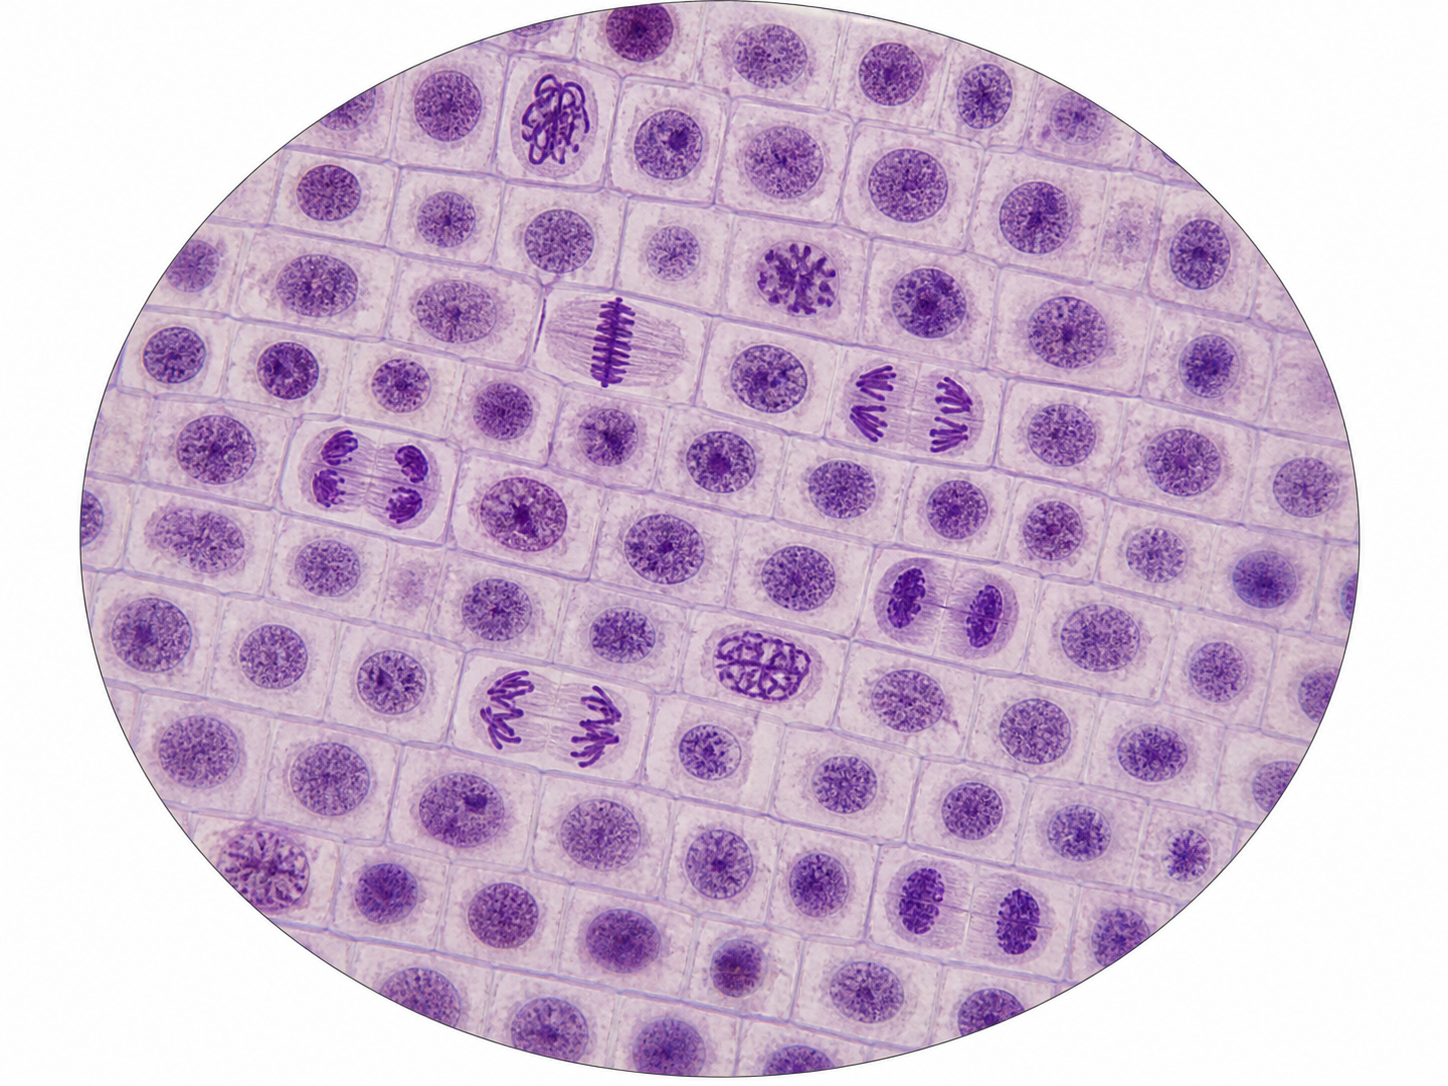
\includegraphics[width=0.58\linewidth]{images/book2/ai/g11-mitosis-root-tip.png}

{\small Un écrasement d'apex de racine d'oignon au microscope optique.
La plupart des \omterm{def:g10:cells-common-unit:cell}{cellules} sont en interphase~; quelques-unes montrent des
\omterm{def:g10:universal-dna:information}{chromosomes} condensés à différents stades de la \omterm{def:g11:cell-cycle-mitosis:cycle}{mitose}. Compter la
proportion de chaque stade mesure la durée de chacun.}
\end{omfigure}

\begin{example}[Compter dans l'apex racinaire]\label{ex:g11:cell-cycle-mitosis:count}
Sur 600 \omterm{def:g10:cells-common-unit:cell}{cellules} comptées dans un apex de racine, 540 sont en
interphase et 60 en \omterm{def:g11:cell-cycle-mitosis:cycle}{mitose}~: un \emph{index mitotique} de 10~\%. Si le
cycle dure 20 heures, la \omterm{def:g11:cell-cycle-mitosis:cycle}{mitose} dure environ
$0.10 \times 20 = \qty{2}{h}$~; et si 36 des 60 \omterm{def:g10:cells-common-unit:cell}{cellules} en division
sont en prophase, la prophase occupe $36/60$ de ces deux heures, soit
quelque 72 minutes, tandis que l'anaphase, vue dans 4 \omterm{def:g10:cells-common-unit:cell}{cellules}
seulement, dure environ 8 minutes. Le stade le plus rare est le plus
rapide.
\end{example}

\begin{method}[Compter chromosomes et chromatides]\label{met:g11:cell-cycle-mitosis:counting}
Pour une \omterm{def:g10:biodiversity-scales:species}{espèce} à $2n$ \omterm{def:g10:universal-dna:information}{chromosomes}~:
\begin{enumerate}
  \item en $\mathrm{G_1}$~: $2n$ \omterm{def:g10:universal-dna:information}{chromosomes}, à une \omterm{def:g11:cell-cycle-mitosis:chromosome}{chromatide} chacun,
        \omterm{def:g10:universal-dna:information}{ADN} $q$~;
  \item après S, pendant $\mathrm{G_2}$, la prophase et la métaphase~:
        $2n$ \omterm{def:g10:universal-dna:information}{chromosomes}, à deux \omterm{def:g11:cell-cycle-mitosis:chromosome}{chromatides} chacun ($4n$ \omterm{def:g11:cell-cycle-mitosis:chromosome}{chromatides}),
        \omterm{def:g10:universal-dna:information}{ADN} $2q$~;
  \item à partir de l'anaphase~: $4n$ \omterm{def:g10:universal-dna:information}{chromosomes} à une \omterm{def:g11:cell-cycle-mitosis:chromosome}{chromatide} dans
        la \omterm{def:g10:cells-common-unit:cell}{cellule}, $2n$ allant vers chaque pôle~;
  \item dans chaque \omterm{def:g10:cells-common-unit:cell}{cellule} fille~: $2n$ \omterm{def:g10:universal-dna:information}{chromosomes}, à une \omterm{def:g11:cell-cycle-mitosis:chromosome}{chromatide}
        chacun, \omterm{def:g10:universal-dna:information}{ADN} $q$.
\end{enumerate}
Une \omterm{def:g11:cell-cycle-mitosis:chromosome}{chromatide} devient un \omterm{def:g11:cell-cycle-mitosis:chromosome}{chromosome} à l'instant où son \omterm{def:g11:cell-cycle-mitosis:chromosome}{centromère} se clive.
\end{method}

\begin{example}[Les nombres humains]\label{ex:g11:cell-cycle-mitosis:human}
Une \omterm{def:g10:cells-common-unit:cell}{cellule} humaine en métaphase détient 46 \omterm{def:g10:universal-dna:information}{chromosomes} et 92
\omterm{def:g11:cell-cycle-mitosis:chromosome}{chromatides}~; en anaphase, 92 \omterm{def:g10:universal-dna:information}{chromosomes}, dont 46 vers chaque pôle~;
chaque fille, 46 \omterm{def:g10:universal-dna:information}{chromosomes} à une \omterm{def:g11:cell-cycle-mitosis:chromosome}{chromatide} chacun, contenant
exactement l'\omterm{def:g10:universal-dna:information}{ADN} que la mère avait au début de son cycle.
\end{example}

\section{À quoi sert la mitose}

\begin{proposition}[La conformité et ses usages]\label{prop:g11:cell-cycle-mitosis:conformity}
Parce que la réplication est fidèle et que la \omterm{def:g11:cell-cycle-mitosis:cycle}{mitose} répartit
exactement les \omterm{def:g11:cell-cycle-mitosis:chromosome}{chromatides}, chaque \omterm{def:g10:cells-common-unit:cell}{cellule} d'un corps pluricellulaire
porte la même \omterm{def:g10:universal-dna:information}{information génétique} que la cellule-œuf dont elle
descend. La \omterm{def:g11:cell-cycle-mitosis:cycle}{mitose} est le mécanisme de la croissance (l'embryon, l'apex
racinaire), du renouvellement (peau, paroi intestinale, sang~: la
seule moelle osseuse fabrique quelque $\num{2e11}$ \omterm{def:g10:cells-common-unit:cell}{cellules} par jour)
et de la réparation (la cicatrisation)~; chez les eucaryotes
unicellulaires, c'est la reproduction elle-même. Son contrôle --- la
décision d'entrer dans le cycle, les vérifications avant S et avant
l'anaphase --- fait l'objet du \cref{ch:g11:cancer}.
\end{proposition}
\admitted

\begin{remark}[Tout ne se divise pas]\label{rem:g11:cell-cycle-mitosis:notall}
La plupart des neurones et des \omterm{def:g10:cells-common-unit:cell}{cellules} du muscle cardiaque quittent le
cycle dans la petite enfance et n'y rentrent jamais~: les dommages
qu'ils subissent ne sont pas réparés par division, et c'est pourquoi
une lésion de la moelle épinière ou un infarctus laisse une perte
durable. Les \omterm{def:g10:cells-common-unit:cell}{cellules} du foie se reposent en $\mathrm{G_1}$ pendant des
mois mais rentrent dans le cycle quand on retire une partie du foie, et
font repousser l'organe en quelques semaines. Quelles \omterm{def:g10:cells-common-unit:cell}{cellules} ont le
droit de se diviser, et quand, est l'une des régulations les plus
strictes du corps.
\end{remark}

\section{Exercices}

\begin{exercise}[$\star$]\label{exo:g11:cell-cycle-mitosis:1}
Nommer les quatre phases du \omterm{def:g11:cell-cycle-mitosis:cycle}{cycle cellulaire} et dire ce qui se passe
dans chacune.
\end{exercise}

\begin{exercise}[$\star$]\label{exo:g11:cell-cycle-mitosis:2}
Définir \omterm{def:g11:cell-cycle-mitosis:chromosome}{chromatide} et \omterm{def:g11:cell-cycle-mitosis:chromosome}{centromère}. Quand un \omterm{def:g11:cell-cycle-mitosis:chromosome}{chromosome} a-t-il deux
\omterm{def:g11:cell-cycle-mitosis:chromosome}{chromatides}~?
\end{exercise}

\begin{exercise}[$\star$]\label{exo:g11:cell-cycle-mitosis:3}
Citer les quatre stades de la \omterm{def:g11:cell-cycle-mitosis:cycle}{mitose} avec un événement clé pour chacun.
\end{exercise}

\begin{exercise}[$\star$]\label{exo:g11:cell-cycle-mitosis:4}
Un \omterm{def:g10:cells-common-unit:organelle}{noyau} contient $1.5q$ d'\omterm{def:g10:universal-dna:information}{ADN}. Dans quelle phase la \omterm{def:g10:cells-common-unit:cell}{cellule} est-elle~?
\end{exercise}

\begin{exercise}[$\star$]\label{exo:g11:cell-cycle-mitosis:5}
Combien de \omterm{def:g10:universal-dna:information}{chromosomes}, et combien de \omterm{def:g11:cell-cycle-mitosis:chromosome}{chromatides}, une \omterm{def:g10:cells-common-unit:cell}{cellule} humaine
a-t-elle en $\mathrm{G_2}$~?
\end{exercise}

\begin{exercise}[$\star\star$]\label{exo:g11:cell-cycle-mitosis:6}
D'après la figure de la quantité d'\omterm{def:g10:universal-dna:information}{ADN}, donner la durée de chaque phase
et dire dans quelles phases on trouverait une \omterm{def:g10:cells-common-unit:cell}{cellule} à $2q$.
\end{exercise}

\begin{exercise}[$\star\star$]\label{exo:g11:cell-cycle-mitosis:7}
Une souris a $2n = 40$. Donner le nombre de \omterm{def:g10:universal-dna:information}{chromosomes} et de
\omterm{def:g11:cell-cycle-mitosis:chromosome}{chromatides} d'une \omterm{def:g10:cells-common-unit:cell}{cellule} en métaphase, en anaphase (\omterm{def:g10:cells-common-unit:cell}{cellule} entière),
et dans une \omterm{def:g10:cells-common-unit:cell}{cellule} fille.
\end{exercise}

\begin{exercise}[$\star\star$]\label{exo:g11:cell-cycle-mitosis:8}
Dans un apex racinaire, on compte 800 \omterm{def:g10:cells-common-unit:cell}{cellules}~: 720 en interphase, 48
en prophase, 16 en métaphase, 6 en anaphase, 10 en télophase. Calculer
l'index mitotique et, pour un cycle de 24 heures, la durée de chaque
stade.
\end{exercise}

\begin{exercise}[$\star\star$]\label{exo:g11:cell-cycle-mitosis:9}
La colchicine, substance extraite du colchique, empêche le fuseau de se
former. Prévoir ce qui arrive à une \omterm{def:g10:cells-common-unit:cell}{cellule} en division qui en est
traitée, et pourquoi les biologistes l'emploient pour préparer des
\omterm{def:g11:cell-cycle-mitosis:chromosome}{caryotypes}.
\end{exercise}

\begin{exercise}[$\star\star$]\label{exo:g11:cell-cycle-mitosis:10}
Expliquer pourquoi les \omterm{def:g10:universal-dna:information}{chromosomes} doivent se condenser avant d'être
déplacés, et pourquoi ils se déroulent ensuite.
\end{exercise}

\begin{exercise}[$\star\star$]\label{exo:g11:cell-cycle-mitosis:11}
Une cellule-œuf se divise toutes les 12 heures les premiers jours.
Combien y a-t-il de \omterm{def:g10:cells-common-unit:cell}{cellules} après 5 jours~? Chaque division
aurait-elle besoin d'une phase $\mathrm{G_1}$ complète~?
\end{exercise}

\begin{exercise}[$\star\star\star$]\label{exo:g11:cell-cycle-mitosis:12}
À l'anaphase, les deux \omterm{def:g11:cell-cycle-mitosis:chromosome}{chromatides} d'un \omterm{def:g11:cell-cycle-mitosis:chromosome}{chromosome} ne se séparent pas
et partent toutes deux vers le même pôle. Décrire les deux \omterm{def:g10:cells-common-unit:cell}{cellules}
filles (nombre de \omterm{def:g10:universal-dna:information}{chromosomes}, \omterm{def:g10:universal-dna:information}{ADN}) et expliquer pourquoi une telle
erreur, dans une \omterm{def:g10:cells-common-unit:cell}{cellule} du corps, est généralement sans conséquence
mais parfois grave.
\end{exercise}

\begin{exercise}[$\star\star\star$]\label{exo:g11:cell-cycle-mitosis:13}
La moelle osseuse fabrique $\num{2e11}$ \omterm{def:g10:cells-common-unit:cell}{cellules} sanguines par jour. Si
une \omterm{def:g10:cells-common-unit:cell}{cellule} précurseur de la moelle boucle son cycle en 24 heures,
estimer combien de précurseurs se divisent à un instant donné, et
commenter l'effet, sur le sang, d'un médicament bloquant la \omterm{def:g11:cell-cycle-mitosis:cycle}{mitose} au
bout d'une semaine.
\end{exercise}

\begin{exercise}[$\star\star\star$]\label{exo:g11:cell-cycle-mitosis:14}
Expliquer pourquoi un \omterm{def:g11:cell-cycle-mitosis:chromosome}{caryotype} est préparé à partir de \omterm{def:g10:cells-common-unit:cell}{cellules}
bloquées en métaphase plutôt qu'en interphase ou en anaphase.
\end{exercise}

\begin{exercise}[$\star\star\star$]\label{exo:g11:cell-cycle-mitosis:15}
On retire les deux tiers d'un foie~; en trois semaines, il a repoussé.
À l'aide du \omterm{def:g11:cell-cycle-mitosis:cycle}{cycle cellulaire}, décrire ce qu'ont fait ses \omterm{def:g10:cells-common-unit:cell}{cellules}, et
dire de quoi avait l'air la teneur en \omterm{def:g10:universal-dna:information}{ADN} des \omterm{def:g10:cells-common-unit:cell}{cellules} hépatiques au
troisième jour par rapport au jour zéro.
\end{exercise}

\section{Problème~: l'emploi du temps d'un apex racinaire}

\begin{problem}[{Problème du week-end --- un apex racinaire compté
cellule par cellule~: la durée de chaque stade du cycle, l'ADN à chaque
instant, les cellules qu'une racine fabrique en un jour, et les huit
minutes de l'anaphase}]
\label{pb:g11:cell-cycle-mitosis:1}
Une classe écrase et colore un apex de racine d'ail ($2n = 16$) et
compte 1000 \omterm{def:g10:cells-common-unit:cell}{cellules} dans la zone de croissance~: 900 en interphase, 60
en prophase, 18 en métaphase, 8 en anaphase, 14 en télophase. Des
mesures indépendantes donnent 20 heures pour le cycle de ces \omterm{def:g10:cells-common-unit:cell}{cellules}.
On admettra que la zone de croissance contient 20\,000 \omterm{def:g10:cells-common-unit:cell}{cellules}.

\medskip
\noindent\textbf{Partie I --- L'index mitotique.}
\begin{enumerate}
  \item Calculer l'index mitotique du tissu.
  \item En admettant que la fraction de \omterm{def:g10:cells-common-unit:cell}{cellules} à un stade donné est
        égale à la fraction du cycle passée à ce stade, calculer la
        durée de la \omterm{def:g11:cell-cycle-mitosis:cycle}{mitose}.
  \item Calculer la durée de chacun des quatre stades.
  \item Quel stade est le plus court~? Proposer pourquoi il peut être
        aussi rapide.
  \item Pourquoi la méthode exige-t-elle de compter beaucoup de
        \omterm{def:g10:cells-common-unit:cell}{cellules}, et pourquoi doivent-elles provenir de la seule zone
        de croissance~?
\end{enumerate}

\medskip
\noindent\textbf{Partie II --- \omterm{def:g10:universal-dna:information}{Chromosomes} et \omterm{def:g10:universal-dna:information}{ADN}.}
\begin{enumerate}[resume]
  \item Combien de \omterm{def:g10:universal-dna:information}{chromosomes}, et combien de \omterm{def:g11:cell-cycle-mitosis:chromosome}{chromatides}, une \omterm{def:g10:cells-common-unit:cell}{cellule}
        d'ail détient-elle en métaphase~?
  \item Combien de \omterm{def:g10:universal-dna:information}{chromosomes} se déplacent dans une \omterm{def:g10:cells-common-unit:cell}{cellule} en
        anaphase, et combien atteignent chaque pôle~?
  \item En appelant $q$ l'\omterm{def:g10:universal-dna:information}{ADN} d'une \omterm{def:g10:cells-common-unit:cell}{cellule} fille, donner la teneur en
        \omterm{def:g10:universal-dna:information}{ADN} d'une \omterm{def:g10:cells-common-unit:cell}{cellule} en prophase, en anaphase (\omterm{def:g10:cells-common-unit:cell}{cellule} entière) et
        en télophase (chaque \omterm{def:g10:cells-common-unit:organelle}{noyau}).
  \item Sur les 900 \omterm{def:g10:cells-common-unit:cell}{cellules} en interphase, combien environ sont en S,
        si $\mathrm{G_1}$, S et $\mathrm{G_2}$ durent 8, 7 et 4
        heures~?
  \item Un élève trouve une \omterm{def:g10:cells-common-unit:cell}{cellule} à 32 \omterm{def:g10:universal-dna:information}{chromosomes} à une \omterm{def:g11:cell-cycle-mitosis:chromosome}{chromatide}
        répartis dans le \omterm{def:g10:cells-common-unit:cell}{cytoplasme}. À quel stade est-elle, et que
        vient-il de se passer~?
\end{enumerate}

\medskip
\noindent\textbf{Partie III --- La production de la racine.}
\begin{enumerate}[resume]
  \item Si chaque \omterm{def:g10:cells-common-unit:cell}{cellule} de la zone de croissance boucle son cycle en
        20 heures, combien de \omterm{def:g10:cells-common-unit:cell}{cellules} neuves la zone produit-elle par
        heure~?
  \item Chaque \omterm{def:g10:cells-common-unit:cell}{cellule} neuve, une fois sortie de la zone de croissance,
        s'allonge jusqu'à environ \qty{100}{\micro m}. Dans une file de
        \omterm{def:g10:cells-common-unit:cell}{cellules} d'une seule \omterm{def:g10:cells-common-unit:cell}{cellule} de large, de combien la racine
        s'allonge-t-elle par jour~? Comparer au \qty{1}{mm} par jour
        observé et expliquer l'écart.
  \item Chaque \omterm{def:g10:cells-common-unit:cell}{cellule} fille doit copier $2n = 16$ \omterm{def:g10:universal-dna:information}{chromosomes}, soit
        quelque $\num{1.6e10}$ paires de \omterm{def:g10:universal-dna:nucleotide}{bases} en tout. Avec des
        fourches à 50 \omterm{def:g10:universal-dna:nucleotide}{nucléotides} par seconde, combien d'origines
        faut-il pour finir dans les 7 heures de la phase S~?
  \item La racine est mise au froid (\qty{4}{\celsius}) pendant un
        jour. Prévoir le changement des comptages, et celui de l'index
        mitotique si le froid ralentit toutes les phases également.
  \item Un herbicide bloque l'\omterm{prop:g11:dna-replication:forks}{ADN polymérase}. Au bout d'un jour, quels
        stades verrait-on encore dans l'écrasement, et lesquels
        auraient disparu~? Expliquer.
\end{enumerate}

\medskip
\noindent\textbf{Partie IV --- Le verdict des comptages.}
\begin{enumerate}[resume]
  \item Une seconde classe compte le même tissu et trouve 4 anaphases
        sur 1000 \omterm{def:g10:cells-common-unit:cell}{cellules}. Quelle durée calcule-t-elle~? Le désaccord
        est-il surprenant pour un stade vu dans une poignée de
        \omterm{def:g10:cells-common-unit:cell}{cellules}~?
  \item En réunissant les deux classes (2000 \omterm{def:g10:cells-common-unit:cell}{cellules}, 12 anaphases),
        recalculer la durée de l'anaphase.
  \item Des \omterm{def:g10:cells-common-unit:cell}{cellules} humaines en culture ont un index mitotique de
        4~\% et un cycle de 24 heures. Comparer la durée de leur \omterm{def:g11:cell-cycle-mitosis:cycle}{mitose}
        à celle de l'ail.
  \item Expliquer pourquoi l'index mitotique d'une tumeur vaut souvent
        plusieurs fois celui du tissu dont elle est issue, et ce que
        cela signifie pour un médicament qui agit sur le fuseau.
  \item Énoncer le résultat~: l'emploi du temps du cycle d'une \omterm{def:g10:cells-common-unit:cell}{cellule}
        de racine d'ail, stade par stade, et le stade dont les huit
        minutes décident que chaque fille reçoit seize \omterm{def:g10:universal-dna:information}{chromosomes}.
\end{enumerate}
\end{problem}
